\documentclass{mini}


\usepackage[utf8x]{inputenc}
\usepackage[T1]{fontenc}
\usepackage[polish]{babel}
\usepackage{indentfirst}
\usepackage{capt-of}
\usepackage{caption}
\usepackage{graphics}
\usepackage{graphicx}
\usepackage{amsmath}
\usepackage{verbatim}
\usepackage{longtable}
\usepackage{array}
\usepackage{listings}
\usepackage[table]{xcolor}
\usepackage{hyperref}
\usepackage[all]{hypcap}
\usepackage{setspace}
\usepackage{indentfirst}

\usepackage[titletoc]{appendix}
\usepackage[colorinlistoftodos]{todonotes}

\usepackage{fancyhdr}
\pagestyle{fancy}
\frenchspacing
\setlength{\parindent}{5mm}
\newcommand*{\myref}[1]{\ref{#1}~--~\textit{\nameref{#1}}}


\lstset{ %
frame=single,           % adds a frame around the code
captionpos=b,
aboveskip=0.75cm,
basicstyle=\ttfamily\small
}

\makeatletter
\def\hlinewd#1{%
\noalign{\ifnum0=`}\fi\hrule \@height #1 %
\futurelet\reserved@a\@xhline}
\makeatother

\usepackage{float} 
\restylefloat{table}

\captionsetup{tablename=Tabela}

\renewcommand\lstlistingname{Fragment kodu}
\renewcommand\lstlistlistingname{Fragmenty kodu}
\def\lstlistingautorefname{Fragm. kodu}


\newcommand{\hiddensubsection}[1]{
    \stepcounter{subsection}
    \subsection*{\arabic{chapter}.\arabic{section}.\arabic{subsection}\hspace{1em}{#1}}
}
\newcommand{\hiddensection}[1]{
    \stepcounter{section}
    \subsection*{\arabic{chapter}.\arabic{section}\hspace{1em}{#1}}
}
\headheight = 13.6pt
 
 
 
 \title{Instrukcja użytkownika}
 
 \titleClass{Reprezentacja wiedzy}

\author{\textbf{Robert Jakubowski}
\\Mariusz Ambroziak
\\Paweł Bielicki
\\Karol Bocian
\\Hanna Dziegciar
\\Karol Dzitkowski
\\Mateusz Jankowski
\\Wiktor Ryciuk}

\supervisor{dr Anna Maria Radzikowska}
 
 \lhead{Reprezentacja wiedzy} % określa lewą część nagłówka
\rhead{Instrukcja użytkownika}


\rfoot{Warszawa \today}

 
\begin{document}



\maketitle


\tableofcontents


\chapter{Aplikacja}
Aplikacja jest realną realizacja scenariuszy działań. Implementuje ona świat, który został opisany w załączonym dokumencie ,,Realizacje scenariuszy działa''. 
Program składa się z trzech głównych widoków oraz jednego pomocniczego. Użytkownik, w przypadku gdy wprowadzi niepoprawne dane, zostanie o tym poinformowany.


\chapter{Widok 1 -- środowisko}

Pierwszym widokiem pojawiającym się po uruchomieniu aplikacji jest widok definiowania środowiska. Jest on przedstawiony na rysunku \ref{fig:1}.
\begin{center}
  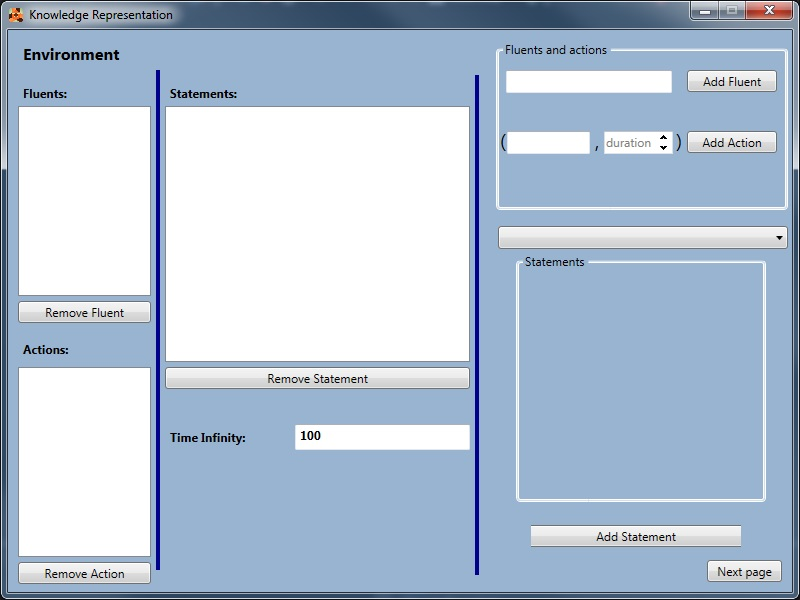
\includegraphics[width=1\textwidth]{1}
   \captionof{figure}{Widok definiowania środowiska.}
   \label{fig:1}
\end{center}

Zaczynając od lewej strony, mamy listę zdefiniowanych fluentów, poniżej listę zdefiniowanych akcji, dalej na prawo listę zdefiniowanych zdań, a pod nim górne ograniczenie czasowe wykonywania się scenariusza. Z każdej z tej listy możemy usunąć już dodany element. W tym celu należy kliknąć na liście element do usunięcia, a następnie nacisnąć przycisk znajdujący się pod tą listą. W celu zmiany ograniczenia czasowego, należy zaznaczyć liczbę znajdującą się obok napisu ,,Time Infinity:'' i zmienić ją na inną. 

Po prawej stronie mamy obszar odpowiedzialny za dodawanie fluentów, akcji oraz wyrażeń. Zaczynając od góry:
w celu dodania fluentu należy wpisać w pole obok przycisku ,,Add Fluent'' nazwę fluentu, a następnie kliknąć przycisk ,,Add Fluent''.
W celu dodania akcji należy wybrać czas trwania akcji w polu  obok przycisku ,,Add Action'',  wpisać nazwę akcji w pole obok pola odpowiadającego długości akcji oraz wybrać przycisk ,,Add Action''.
W celu dodania zdania należy z listy rozwijanej wybrać interesujące nas wyrażenie. Obszar ,,Statement'' wypełni się kontrolkami odpowiednimi dla danego wyrażenia. Są tam pola trzech rodzajów, tj. lista rozwijana zawierająca zdefiniowane akcje lub fluenty, numeryczne pole do wyboru czasu oraz pole do wyboru wyrażenia  (zostało ono zdefiniowane w punkcie \myref{chap:pom}). Po wypełnieniu wszystkich pól należy kliknąć przycisk ,,Add Statement''.

Po zdefiniowaniu środowiska, należy przejść do następnego widoku klikając w przycisk ,,Next Page''.

\chapter{Widok pomocniczy -- wyrażenie}
\label{chap:pom}

Rysunek \ref{fig:4} przedstawia widok umożliwiający definiowanie wyrażeń.

\begin{center}
  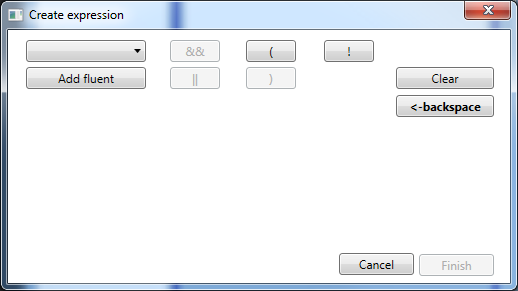
\includegraphics[width=1\textwidth]{4}
   \captionof{figure}{Widok do wprowadzania wyrażeń.}
   \label{fig:4}
\end{center}

W celu dodania wyrażenia możemy:
wybrać z listy interesujący nas fluent, a potem zatwierdzić go przyciskiem ,,Add fluent'' lub wybrać inne przyciski odpowiadające wartościom, które przedstawiają ich napisy. 
Okno zawiera przycisk ,,Clear'' odpowiadający za skasowanie całego tworzonego wyrażenie oraz przycisk ,,<-backspace'' odpowiadający za skasowanie ostatniego wprowadzonego słowa.

Okno możemy opuścić poprzez przycisk ,,Cancel'', który sprawi, że tworzone wyrażenie nie zostanie zapisane, lub przez przycisk ,,Finish'', który zachowa stworzone wyrażenie.



\chapter{Widok 2 -- scenariusze}

Rysunek \ref{fig:2} przedstawia widok umożliwiający definiowanie scenariuszy.

\begin{center}
  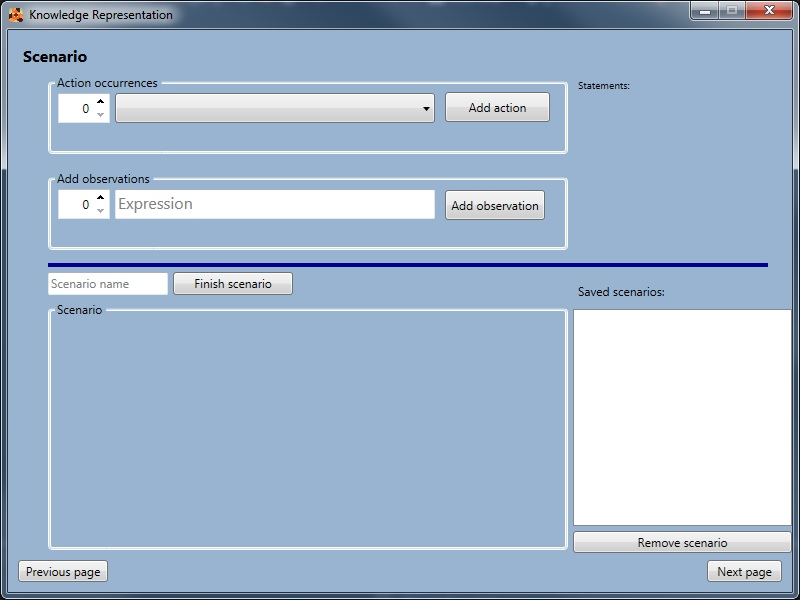
\includegraphics[width=1\textwidth]{2}
   \captionof{figure}{Widok do wprowadzania scenariuszy.}
   \label{fig:2}
\end{center}

Począwszy od góry mamy: dodawanie akcji, poprzez wpisanie czasu jej wystąpienia oraz wybrania jej z listy rozwijanej, a następnie kliknięciu  przycisku ,,Add action''.
Poniżej mamy możliwość dodawania wyrażeń przez wybranie czasu jego wystąpienia oraz kontrolkę ,,Expression''. Następnie należy kliknąć przycisk ,,Add expression''.
Poniżej jest pole do wpisania nazwy scenariusza, a obok przycisk ,,Finish scenario'', który dodaje scenariusz do listy scenariuszy oraz kończy jego definiowanie.
Poniżej znajduje się lista zdefiniowanych akcji i wyrażeń w tworzonym scenariuszu. W prawej kolumnie mamy listę dostępnych wyrażeń, a poniżej listę zdefiniowanych scenariuszy. Po wybraniu odpowiedniego, możemy go skasować używając przycisku ,,Remove scenario''.

W celu przejścia do następnego widoku należy nacisnąć przycisk ,,Next page''. Przycisk ,,Previous page'' umożliwia powrót do poprzedniego widoku. 

\chapter{Widok 3 -- kwerendy}

Rysunek \ref{fig:2} przedstawia widok umożliwiający definiowanie kwerendy oraz uruchamiania jej.

\begin{center}
  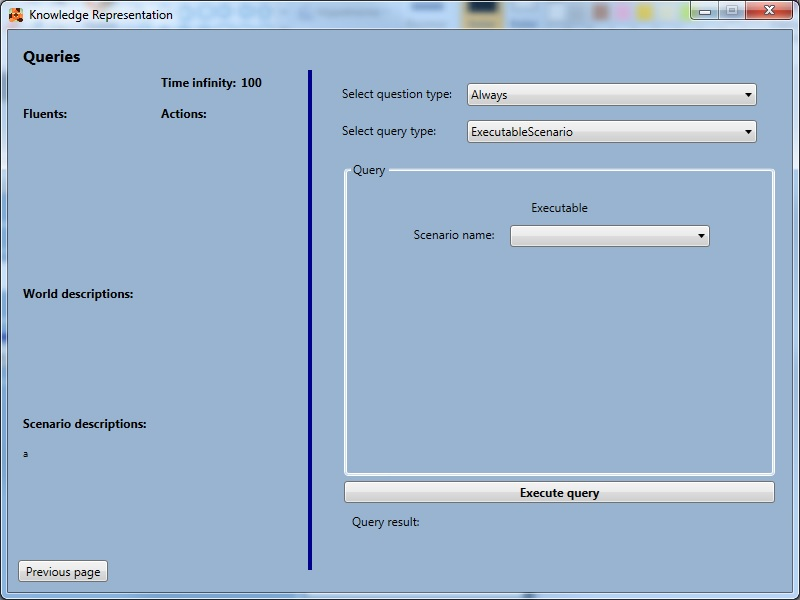
\includegraphics[width=1\textwidth]{3}
   \captionof{figure}{Widok do definiowania kwerendy.}
   \label{fig:3}
\end{center}

Po lewej stronie mamy kolejno: ograniczenie czasowe, listę zdefiniowanych fluentów, akcji, opisów świata oraz scenariuszy.
Z prawej strony jest lista rozwijana do wyboru typu pytania, a poniżej wybór typu kwerendy. Po wybraniu odpowiedniego typu kwerendy, obszar ,,Query'' ulegnie zmianie, w celu zdefiniowania szczegółów danej kwerendy. Pojawia się znane już pola typu: wprowadź wyrażenie, podaj czas oraz lista rozwijana ze zdefiniowanymi scenariuszami.
Poniżej jest przycisk ,,Execute query'', który uruchamia zdefiniowaną kwerendę. Wynik wyświetli się obok napisu ,,Query result''.

Przycisk ,,Previous page'' umożliwia powrót do poprzedniego widoku.




\end{document}